\documentclass{article}
\usepackage[utf8]{inputenc}
\usepackage{polski}
\usepackage[polish]{babel}
\usepackage{bbm}
\usepackage{amsmath}
\usepackage{amsthm}
\usepackage{graphicx}
\usepackage{epstopdf}
\usepackage{float}

\newtheorem{defi}{Definicja}
\newtheorem{twr}{Twierdzenie}
\newtheorem*{dd}{Dowód}

\DeclareMathOperator{\sign}{sign}
\DeclareMathOperator{\arctg}{arctg}

\newcommand{\twopartdef}[4]
{
	\left\{
		\begin{array}{ll}
			#1 & \mbox{jeśli } #2 \\
			#3 & \mbox{jeśli } #4
		\end{array}
	\right.
}


\author{Jarosław Dzikowski 273233}
\date{Wrocław, \today}
\title{\textbf{Pracownia z analizy numerycznej} \\ Sprawozdanie do zadania \textbf{P.2.9}}
\begin{document}
\maketitle
\section{Uwagi techniczne}
Program można uruchomić normalnie z wiersza poleceń. Nie wypisuje on dużo, ponieważ wyniki doświadczeń są zamieniane na wykresy. Program ma zakomentowane wywołania funkcji produkującej dane do sporządzenia wykresu przez gnuplot'a.\\

Sprawozdanie należy kompilować z wiersza poleceń będąc wewnątrz katalogu doc.
Do skompilowania sprawozdania wymagana jest obecność folderu ,,wykresy'' z wykresami w formacie eps, które następnie będą zamieszczone w sprawozdaniu. Folder ,,wykresy'' znajduje się w folderze ,,doc''.

\section{Wstęp}
W tym zadaniu pochylimy się nad interpolacją Lagrange'a. Sprawdzimy zależność między wskaźnikiem uwarunkowania interpolacji a jej błędem względnym. Następnie doświadczalnie sprawdzimy wspomniane zależności na przykładzie kilku funkcji.
Wszystkie nasze badania będą przeprowadzone w przedziale $[-1, 1]$.

\section{Wprowadzenie}

\subsection{Zagadnienie interpolacji}
Weźmy funkcję $f$. Obliczenia na tej funkcji (Np. całkowanie) mogą być bardzo trudne do policzenia. Dlatego chcielibyśmy skonstruować w zadanym przedziale $[x_0, x_n]$ prostszą funkcję $L_n$, wielomian, która zachowuje się podobnie do $f$ oraz przyjmuje takie same wartości w punktach $x_i$ dla ($i = 0, 1, ... , n$). Punkty te będziemy nazywać \emph{węzłami interpolacji}. Skoro $L_n$ przybiera określone wartości w $n+1$ punktach, to $L_n \in \Pi_n$, gdzie $\Pi_n$ to przestrzeń wielomianów stopnia $n$.

\begin{defi}[Wielomian interpolacyjny Lagrange'a]

Niech $x_0, x_1, ... , x_n$ będą węzłami interpolacji funkcji $f$. Wielomianem Lagrange'a interpolującym $f$ nazwiemy $L_n$, takie że:
\begin{equation}
L_n(x) = \sum_{k = 0}^n \lambda_k(x) f(x_k)
\end{equation}
gdzie $\lambda_k(x)$ wyraża się wzorem:
\begin{equation}
\lambda_k(x) = \prod_{\substack{j = 0 \\ j \neq k}}^n \frac{(x - x_j)}{(x_k - x_j)}
\end{equation}

\end{defi}

\begin{twr}
Niech $L_n \in \Pi_n$ będzie wielomianem interpolacyjnym Lagrange'a w węzłach $x_0, x_1, ..., x_n$. Wtedy mamy:
\begin{equation*}
L_n(x_i) = f(x_i) , (i = 0, 1, ..., n)
\end{equation*}
\end{twr}

\begin{dd}
\normalfont
Weźmy dowolne $i \in \{0, 1, ..., n\}$. Wiemy, że
\begin{equation*}
L_n(x_i) = \sum_{k = 0}^n \lambda_k(x_i) f(x_k)
\end{equation*}
Przyjrzyjmy się wartości $\lambda_k(x_i)$:
\begin{equation*}
\lambda_k(x_i) = \prod_{\substack{j = 0 \\ j \neq k}}^n \frac{(x_i - x_j)}{(x_k - x_j)}
\end{equation*}
Można zatem zauważyć, że dla $i \neq k$ i $j = i$ liczniku znajduje się czynnik $(x_i - x_j) = (x_j - x_j) = 0$. Natomiast dla $i = k$ i dowolnego $j \neq k$ mamy czynnik $\frac{(x_i - x_j)}{(x_k - x_j)} = \frac{(x_k - x_j)}{(x_k - x_j)} = 1$. Zatem
\begin{equation*}
\lambda_k(x_i) = \twopartdef {0} {i \neq k} {1} {i = k}
\end{equation*}
W takim wypadku
\begin{equation*}
L_n(x_i) = \sum_{k = 0}^n \lambda_k(x_i) f(x_k) = \lambda_i(x_i) f(x_i) = f(x_i)
\end{equation*}
\qed
\end{dd}

\subsection{Wskaźnik uwarunkowania}
Niech $A$ będzie algorytmem obliczającym rzeczywisty wynik dla danych $X$, $A(X)$. Wskaźnik uwarunkowania $K$ mowi jak duży może być błąd względny algorytmu $A$ w stosunku do błędu względnego danych $X$.
\begin{equation*}
\frac{|A(X) - \bar{A}(X)|}{|A(X)|} \approx \delta K
\end{equation*}
gdzie $\bar{A}(X)$ jest wynikiem algorytmu A dla zaburzonych danych $X$, a $\delta$ jest błędem względnym danych wejściowych $X$.
\\
Powiemy, że algorytm jest \emph{źle uwarunkowany} dla danych $X$ jeśli wskaźnik uwarunkowania $K$ jest duży (Dąży do nieskońzoności etc.). Wtedy nawet mały błąd względny danych wyprodukuje nam ogromy błąd względny wyniku algorytmu.\\
Jeśli dla danych wejściownych $X$ wskaźnik uwarunkowania $K$ jest mały, to algorytm jest \emph{dobrze uwarunkowany} dla danych $X$.

\subsection{Wskaźnik uwarunkowania interpolacji Lagrange'a}
Wyprowadźmy wzór na wskaźnik uwarunkowania interpolacji Lagrange'a.
\begin{twr}[Wskaźnik uwarunkowania interpolacji Lagrange'a]
Niech $L_n \in \Pi_n$ będzie wielomianem Lagrange'a interpolującym funkcję $f$ w węzłach $x_0, x_1, ..., x_n \in [-1, 1]$, wyrażającym się wzorem
\begin{equation*}
\sum_{k = 0}^n \lambda_k(x) f(x_k)
\end{equation*}
Wtedy wskaźnik uwarunkowania interpolacji Lagrange'a $K_n$ wyraża się wzorem
\begin{equation}
K_n = \max_{-1 \leq x \leq 1} \sum_{k = 0}^n |\lambda_k(x)|
\end{equation}
\end{twr}

\begin{dd}
\normalfont
Aby wyprowadzić wskaźnik uwarunkowania należy oszacować z góry bład względny interpolacji funkcji $f$ wielomianem $L_n$ w zależności od błędu względnego danych wejściowych $\delta$. Zastanówmy się jednak, co w przypadku interpolacji będzie naszymi danymi wejściowymi. Wydaje się oczywiste, że za dane posłużą nam węzły interpolacji $x_0, x_1, ..., x_n$. Jednak zauważmy, że tak naprawdę dostajemy $n+1$ par $(x_i, f(x_i))$, więc możemy także potraktować jako dane wartości funkcji $f$ w węzłach.\\
Mając ustalone, czym są nasze dane wejściowe, możemy zacząć szacować błąd względny interpolacji:
\begin{equation*}
\frac{|L_n(x) - \bar{L}_n(x)|}{|L_n(x)|} = \frac{|\sum_{k = 0}^n \lambda_k(x) f(x_k) - \sum_{k = 0}^n \lambda_k(x) \bar{f}(x_k)|}{|\sum_{k = 0}^n \lambda_k(x) f(x_k)|} = 
\end{equation*} 
\begin{equation*}
 = \frac{|\sum_{k = 0}^n \lambda_k(x) f(x_k) - \sum_{k = 0}^n \lambda_k(x) f(x_k) (1 + \delta_k)|}{|\sum_{k = 0}^n \lambda_k(x) f(x_k)|} = \frac{|\sum_{k = 0}^n \lambda_k(x) \delta_k f(x_k)|}{|\sum_{k = 0}^n \lambda_k(x) f(x_k)|} 
\end{equation*} 
Możemy teraz skorzystać z nierówności trójkąta
\begin{equation*}
\frac{|\sum_{k = 0}^n \lambda_k(x) \delta_k f(x_k)|}{|\sum_{k = 0}^n \lambda_k(x) f(x_k)|} \leq \frac{\sum_{k = 0}^n |\lambda_k(x) \delta_k f(x_k)|}{|\sum_{k = 0}^n \lambda_k(x) f(x_k)|} 
\end{equation*}
Następnie każdy błąd względny danych $\delta_k$ możemy oszacować z góry przez $\delta = \max |\delta_k|$. Stąd otrzymujemy
\begin{equation*}
\frac{\sum_{k = 0}^n |\lambda_k(x) \delta_k f(x_k)|}{|\sum_{k = 0}^n \lambda_k(x) f(x_k)|} \leq \delta \frac{\sum_{k = 0}^n |\lambda_k(x) f(x_k)|}{|\sum_{k = 0}^n \lambda_k(x) f(x_k)|} 
\end{equation*}
Możemy posunąć się z naszym szacowaniem jeszcze dalej. Niech $F_n$ będzie największą spośród wartości funkcji $f$ w węzłach $x_0, x_1, ..., x_n$. Zatem mamy
\begin{equation*}
\delta \frac{\sum_{k = 0}^n |\lambda_k(x) f(x_k)|}{|\sum_{k = 0}^n \lambda_k(x) f(x_k)|} \leq \delta \frac{\sum_{k = 0}^n |\lambda_k(x) F|}{|\sum_{k = 0}^n \lambda_k(x) F|} = \delta \frac{\sum_{k = 0}^n |\lambda_k(x)|}{|\sum_{k = 0}^n \lambda_k(x)|} 
\end{equation*}
Na mocy zadania 5.1, podpunkt a) wiemy, że $\sum_{k = 0}^n \lambda_k(x) = 1$. Skorzystamy z tego faktu w naszym szacowaniu:
\begin{equation*}
\delta \frac{\sum_{k = 0}^n |\lambda_k(x)|}{|\sum_{k = 0}^n \lambda_k(x)|} = \delta \frac{\sum_{k = 0}^n |\lambda_k(x)|}{1} = \delta \sum_{k = 0}^n |\lambda_k(x)|
\end{equation*}
Ponieważ rozpatrujemy interpolację funkcji $f$ w przedziale $[-1, 1]$, możemy na sam koniec wykonać ostatnie szacowanie:
\begin{equation*}
\delta \sum_{k = 0}^n |\lambda_k(x)| \leq \delta \max_{-1 \leq x \leq 1}  \sum_{k = 0}^n |\lambda_k(x)|
\end{equation*}
Ostatecznie mamy
\begin{equation*}
\frac{|L_n(x) - \bar{L}_n(x)|}{|L_n(x)|} \leq \delta \max_{-1 \leq x \leq 1}  \sum_{k = 0}^n |\lambda_k(x)|
\end{equation*}
Stąd bierzemy wskaźnik uwarunkowania
\begin{equation*}
K_n = \max_{-1 \leq x \leq 1}  \sum_{k = 0}^n |\lambda_k(x)|
\end{equation*}
\qed
\end{dd}

\subsection{Interpolacja Lagrange'a jako przekształcenie liniowe}
Rozważmy przestrzeń funkcji rzeczywistych $F_{\mathbbm{R}}$ oraz ustalone węzły interpolacji. Wtedy interpolacja Lagrange'a $L_n$ jest przekształceniem liniowym z przestrzeni funkcji rzeczywistych do przestrzeni wielomianów stopnia co najwyżej n-tego.
\begin{equation*}
L_n : F_{\mathbbm{R}} \to \Pi_n
\end{equation*}
Oczywistym jest, że trzy własności przekształcenia liniowego zachodzą:
\begin{enumerate}
\item 
\begin{equation*}
L_n 0 = 0
\end{equation*}
\item 
\begin{equation*}
L_n (f+g) = L_n f + L_n g
\end{equation*}
\item 
\begin{equation*}
L_n (\alpha f) = \alpha L_n f \quad (\alpha \in \mathbbm{R})
\end{equation*}

\end{enumerate}

Można także zauważyć, że $L_n$ jest rzutem, tj
\begin{equation*}
L_n^2 = L
\end{equation*}
Można to udowodnić w sposób następujący: niech $v \in \Pi_n$ oraz $v = L_n f$. Wtedy $L_n v = L_n^2 f$. Ponieważ $v \in \Pi_n$, $v$ interpoluje sam siebie. Zatem $L_n v = v$ i stąd $L_n^2 f = L_n f$.\\
Zarówno $F_{\mathbbm{R}}$ jak i $\Pi_n$ są przestrzeniami liniowymi unormowanymi, gdzie normę przekształcenia liniowego możemy określić w sposób następujący. Niech $T$ będzie przekształceniem liniowym w przestrzeni unormowanej.
\begin{equation*}
||T|| = \sup_{||f|| \le 1} \{||T f||\}
\end{equation*}
Oczywiście zachodzi $||Tf|| \le ||T||\ ||f||$.
Jeśli $||T|| < \infty$, to mówimy, że $T$ jest ograniczone.\\

Niech $V$ będzie unormowaną przestrzenią liniową oraz $v \in V$. Niech $W < V$. Wtedy odległością wektora $v$ od podprzestrzeni $W$ zdefiniujemy w taki sposób
\begin{equation*}
dist(v, W) = \inf_{w \in W} \{||v - w||\}
\end{equation*}
\begin{twr}[Odległość między rzutem na podprzestrzeń a wektorem]
Niech $W < V$ oraz $P : V \to W$ będzie ograniczonym rzutem, tj. $||P|| < \infty$ i $P^2 = P$. Wtedy zachodzi nierówność
\begin{equation*}
||v - Pv|| \le ||I - P|| \ dist(v, W) \le (1 + ||P||) \ dist(v, W)
\end{equation*}
\end{twr}
\begin{dd}
\normalfont 
Weźmy dowolny wektor $w \in W$. Ponieważ $Pw = w$ mamy
\begin{equation*}
||v - Pv|| = ||(v - w) - P(v - w)|| = ||(I - P)(v - w)|| \le ||I - P|| \ ||v - w|| \le 
\end{equation*}
możemy teraz dobrać $w$ takie, że norma będzie jak najmniejsza
\begin{equation*}
 \le ||I - P|| \ dist(v, W) \le (1 + ||P||) \ dist(v, W)
\end{equation*} 
\qed
\end{dd}
Powyższe twierdzenie można wykorzystać w kontekscie interpolacji Lagrange'a. Wiemy już, że $L_n$ jest rzutem na przestrzeń wielomianów stopnia co najwyżej n-tego $\Pi_n$. Możemy stąd ograniczyć błąd interpolacji. Niech $p_n^{*} \in \Pi_n$ będzie wielomianem optymalnym dla funkcji $f$, tj. 
\begin{equation*}
\forall_{p_n \in \Pi_n} \ ||f - p_n^{*}|| \le ||f - p_n||
\end{equation*} 
Wtedy mamy
\begin{equation*}
||f - L_n f|| \le (1 + ||L_n||) \ ||f - p_n^{*}||
\end{equation*}


\section{Stała Lebesgue'a}

\begin{defi}
Niech $x_0, x_1, ..., x_n \in [-1, 1]$, a $\lambda_k(x) = \prod_{\substack{j = 0\\j \neq k}}^n \frac{(x - x_j)}{(x_k - x_j)} $.
Definiujemy funkcję Lebesgue'a $l_n : [-1, 1] \to \mathbbm{R}$ w sposób następujący
\begin{equation*}
l_n(x) = \sum_{k = 0}^n |\lambda_k(x)|
\end{equation*}
Natomiast stałą Lebesgue'a definiujemy jako 
\begin{equation*}
\Lambda_n = \max_{-1 \leq x \leq 1} l_n(x) = \max_{-1 \leq x \leq 1} \sum_{k = 0}^n |\lambda_k(x)|
\end{equation*}
\end{defi}

Funkcja oraz stała Lebesgue'a zależą od doboru węzłów $X = \{x_0, x_1, ... x_n \}$. $\Lambda_n(X)$ będzie oznaczało stałą Lebesgue'a dla węzłów $X$. W dalszej części sprawozdania przedstawione zostaną zależności stałej Lebesgue'a od wyboru węzłów.

\begin{twr}[Norma interpolacji Lagrange'a]
Dla ustalonych węzłów interpolacji normą interpolacji Lagrange'a jest stała Lebesgue'a
\begin{equation*}
||L_n|| = \Lambda_n
\end{equation*}
\end{twr}
\begin{dd}
\normalfont
Udowodnimy powyższą równość wykazując dwie nierówności. Dla $||f|| < 1$ mamy
\begin{equation*}
||L_n f|| = \sup_{x \in \mathbbm{R}} |(L_n f)(x)| = \sup_{x \in \mathbbm{R}} \left| \sum_{j = 0}^n f(x_j)\lambda_j(x)\right| \le
\end{equation*}
Z nierówności trójkąta
\begin{equation*}
\le \sup_{x \in \mathbbm{R}} \sum_{j = 0}^n |f(x_j)| \ |\lambda_j(x)| \le \sup_{x \in \mathbbm{R}} \sum_{j = 0}^n |\lambda_j(x)| = \Lambda_n
\end{equation*}
Żeby wykazać nierówność w drugą stronę obierzemy punkt $\zeta$, taki że $l_n(\zeta) = \Lambda_n$. Teraz weźmy funkcję $f$, taką że $||f|| = 1$ i $f(x_j) = \sign \lambda_j(\zeta)$. Zauważmy, że dla tak zdefiniowanego $f$ mamy
\begin{equation*}
||L_n|| \ge ||L_n f|| \ge (L_n f)(\zeta) = \sum_{j = 0}^n f(x_j)\lambda_j(\zeta) = \sum_{j = 0}^n |\lambda_j(\zeta)| = l_n(\zeta) = \Lambda_n
\end{equation*}
\qed
\end{dd}
Możemy teraz sformułować nast. twierdzenie.
\begin{twr}[O ograniczeniu błędu interpolacji]
Niech $L_n$ interpoluje funkcję $f$ w punktach $x_0, x_1, ..., x_n$. Wtedy błąd interpolacji można ograniczyć z góry przez 
\begin{equation}
||f - L_n f|| \le (\Lambda_n + 1) \ ||f - p_n^{*}||
\end{equation}
gdzie $p_n^{*}$ jest optymalnym wielomianem n-tego stopnia dla funkcji $f$.
\end{twr}
Dowód tego twierdzenia polega na przytoczeniu twierdzenia o ograniczeniu odległości między wektorem a jego rzutem na podprzestrzeń wstawiając jako rzut $P$ interpolację Lagrange'a $L_n$. Normę $||L_n||$ znamy z wcześniej udowodnionego twierdzenia.\\

\begin{twr}[Erdo\"s, Brutman] Stała Lebesgue'a spełnia nierówność
\begin{equation*}
\Lambda_n(X) > \frac{2}{\pi}\log n + 0.5212
\end{equation*}
\end{twr}
Oryginalny artykuł autorstwa Erdo\"sa [3] zawierał poprawny czynnik $\frac{2}{\pi}$, lecz błędną stałą. Dopiero Brutman [4] udowodnił powyższe twierdzenie.

\subsection{Węzły równoodległe}
\begin{figure}[H]
	\centering
    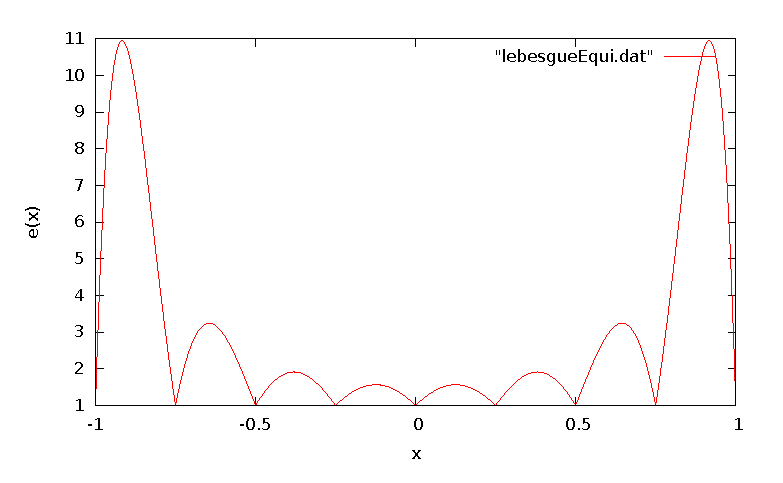
\includegraphics[width=0.8\textwidth]{wykresy/lebesgueEqui.eps}
    \caption{Funkcja Lebesgue'a w węzłach równoodległych (n = 9)}
\end{figure}
Niech $X$ będzie zbiorem węzłów równoodłegłych w przedziale $[-1, 1]$: $x_i = \frac{2i}{n} - 1$, $i = 0, 1, ..., n$. Turetskii [6] wykazał, że dla węzłów równoodległych stała Lebesgue'a spełnia
\begin{equation*}
\Lambda_n(X) \sim \frac{2^n}{en\log n}
\end{equation*}
gdzie $\sim$ oznacza ,,rośnie proporcjonalnie''. W porównaniu do efektów, które uzyskamy dla innego doboru węzłow, wynik ten nie prezentuje się zbyt dobrze.

\subsection{Węzły Czybyszewa}
\begin{figure}[H]
	\centering
    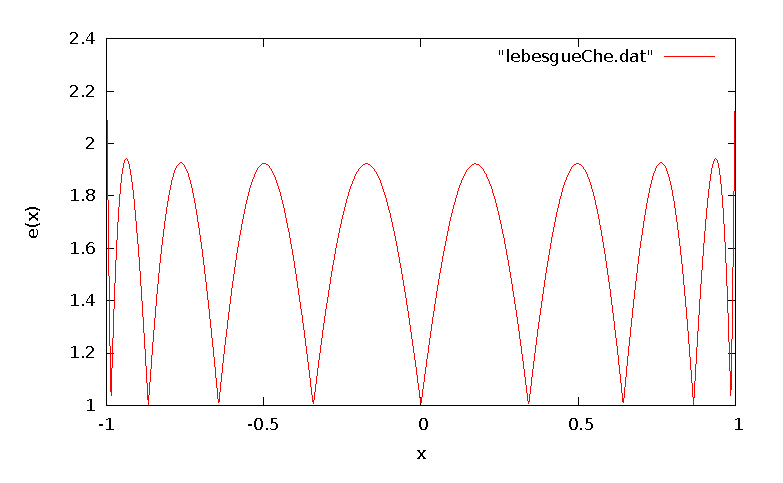
\includegraphics[width=0.8\textwidth]{wykresy/lebesgueChe.eps}
    \caption{Funkcja Lebesgue'a w węzłach Czybyszewa (n = 9)}
\end{figure}
Wielomiany Czybyszewa wyrażają się następujacą zależnością rekurencyna:
\begin{equation*}
T_0 \equiv 1
\end{equation*}
\begin{equation*}
T_1(x) = x
\end{equation*}
\begin{equation*}
T_{n+2}(x) = 2x \cdot T_{n+1}(x) - T_n(x)
\end{equation*}
W przedziale $[-1, 1]$ wielomiany Czybyszewa wyrażają się wzorem
\begin{equation*}
T_n(x) = \cos(n \cdot \arccos(x))
\end{equation*}
To pozwala nam wyznaczyć wzory na miejsca zerowe wielomianu Czybyszewa w przedziale $[-1, 1]$. Niech ${t_n}_i$ będzie i-tym miejscem zerowym wielomianu $T_n$. Wtedy ${t_n}_i$ wyraża sie wzorem
\begin{equation}
{t_n}_i = \cos \frac{(2i - 1)}{n} \frac{\pi}{2}
\end{equation}
Następnie obierzmy miejsca zerowe ${t_n}_i$ n-tego wielomianu Czybyszewa jako węzły interpolacji. Okazuje sie, że dla tak obranych węzłow następujące twierdzenie Rivlina [5] jest prawdziwe:
\begin{twr}
Niech $T$ będzie węzłami w zerach n-tego wielomianu Czybyszewa. Wtedy zachodzi nierówność
\begin{equation*}
0.9625 + \frac{2}{\pi}\log n < \Lambda_n(T) < 1 + \frac{2}{\pi} \log n
\end{equation*}
\end{twr}

\subsection{Rozszerzone węzły Czybyszewa}
\begin{figure}[H]
	\centering
    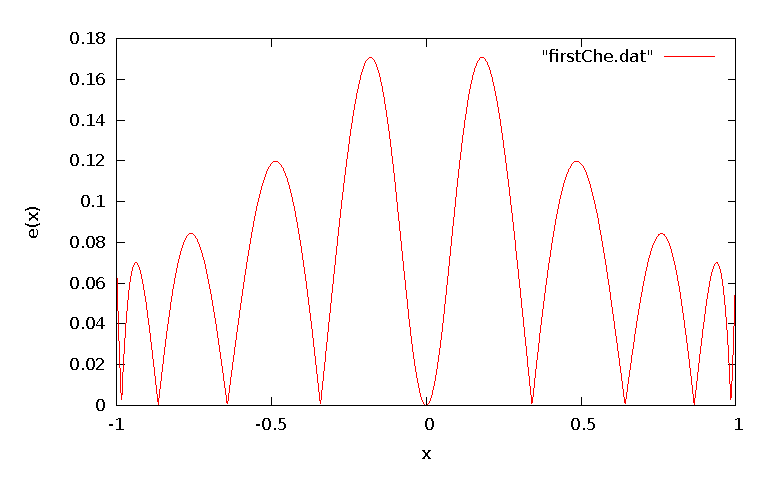
\includegraphics[width=0.8\textwidth]{wykresy/firstChe.eps}
    \caption{Funkcja Lebesgue'a dla rozszerzonych węzłów Czybyszewa (n = 9)}
\end{figure}
Rozszerzone węzły Czybyszewa (\emph{ang. extended Chebyshev nodes}) $\hat{T}$ definiuje się następująco
\begin{equation*}
\hat{T} = \{{x_n}_k = \cos[(2k - 1)\pi/(2n)] / \cos[\pi/(2n)] : k = 0\}
\end{equation*}
Węzły Czybyszewa zostały przeskalowane tak, żeby dla każdego $n$ największe węzły co do modułu były równe $\pm 1$. Mamy
\begin{equation*}
x_1 = \frac{\cos[(2 \cdot 1 - 1) \pi/(2n)]}{cos[\pi/(2n)]} = +1 \quad x_n = \frac{\cos[(2 \cdot n - 1) \pi/(2n)]}{cos[\pi/(2n)]} = -1
\end{equation*}
Przyglądając się funkcji Lebesgue'a dla rozszerzonych węzłow zauważamy, że jest ona taka jak dla zwykłych węzłów Czybyszewa, ale w punkach pomnożonych przez $\cos[\pi/(2n)]$
\begin{equation*}
l_n(\hat{T}, x) = l_n(T, x \cos[\pi/(2n)])
\end{equation*}
Dla rozszerzonych węzłów Czybyszewa wykazano, że stała Lebesgue'a ma następującą asymptotykę:
\begin{equation*}
\Lambda_n(\hat{T}) = \frac{2}{\pi} \log n + \frac{2}{\pi}\Big(\gamma + \log \frac{8}{\pi} - \frac{2}{3}\Big) + O \Big(\frac{1}{\log n}\Big)
\end{equation*}

\subsection{Węzły optymalne}
Dobór węzłów optymalnych, dla których stała Lebesgue'a będzie minimalna pozostaje problemem otwartym. Jednakże, można oszacować od dołu optymalną stałą Lebesgue'a. Niech $\Lambda_n^* = \min_{X} \Lambda_n(X)$.
Faber [7] w swoim artykule oszacował od dołu $\Lambda_n^*$
\begin{equation*}
\Lambda_n^* > \frac{\log n}{8 \sqrt{\pi}}
\end{equation*}
Z kolei w swoim artykule Vertesi wykazał następującą asymptotykę stałej Lebesgue'a dla optymalnych węzłów
\begin{equation*}
\Lambda_n^* = \frac{2}{\pi} \log n + \frac{2}{\pi} \Big( \gamma + \log {4}{\pi}\Big) + O\left(\left(\frac{\log \log n}{\log n}\right)^2\right)
\end{equation*}


\section{Doświadczenia}
W tej sekcji zostaną opisane wyniki przeprowadzonych doświadczeń. Policzymy wskaźnik uwarunkowania interpolacji w zależności od dobranych węzłów. Zbadamy jak ma się wskaźnik uwarunkowania do dokładności przybliżenia funkcji. Wszystkie przedstawione wykresy zostały wygenerowane za pomocą programu i gnuplota.
Do doświadczeń będziemy używać trzech funkcji:
\begin{equation*}
f_1(x) = \frac{1}{1 + 25x^2} \ f_2(x) = \arctg x \ f_3(x) = \max(0, 1 - 4x)
\end{equation*}
Oczywiście, im więcej węzłów, tym dokładniejsza jest interpolacja. Dlatego my obierzemy sobie małe $n$, w naszych doświadczeniach $n = 9$.

\subsection{Węzły równoodległe}
Mamy do czynienie z $n$ węzłami równoodległymi w przedziale $[-1,1]$. Stała Lebesgue'a przy $n = 9$ węzłach równoodległych wynosi
\begin{equation*}
\Lambda_n = 10.945005461386044
\end{equation*}
Poniżej znajduje się zamieszczony wykres stałej Lebesgue'a w przedziale [5,20].
\begin{figure}[H]
    \centering
    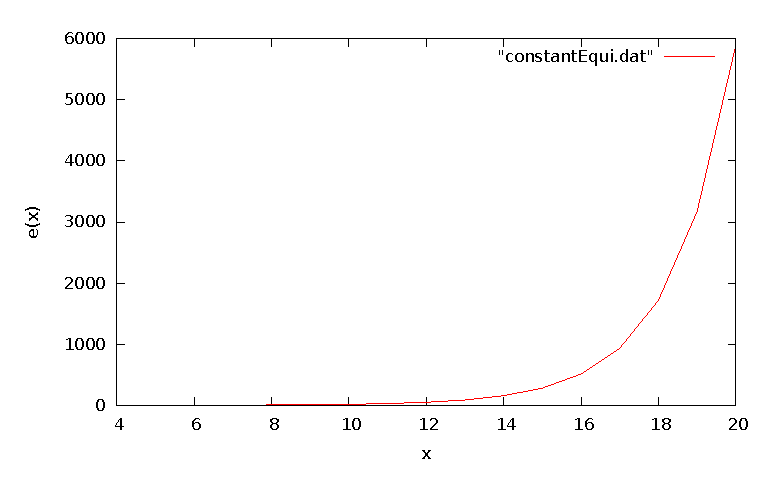
\includegraphics[width=0.8\textwidth]{wykresy/constantEqui.eps}
    \caption{Wykres stałej Lebesgue'a dla węzłów równoodległych}
\end{figure}
Wykres ten potwierdza wykładniczy wzrost stałej $\Lambda_n$.
Jak można było zobaczyć na wykresie funkcji Lebesgue'a dla węzłów równoodległych w poprzedniej sekcji wartości funkcji wewnątrz przedziału są stosunkowo małe, lecz na krańcach przedziału gwałtownie wzrastają.
\begin{enumerate}
\item $f_1(x) = \frac{1}{1 + 25x^2}$\\
\begin{figure}[H]
	\centering
    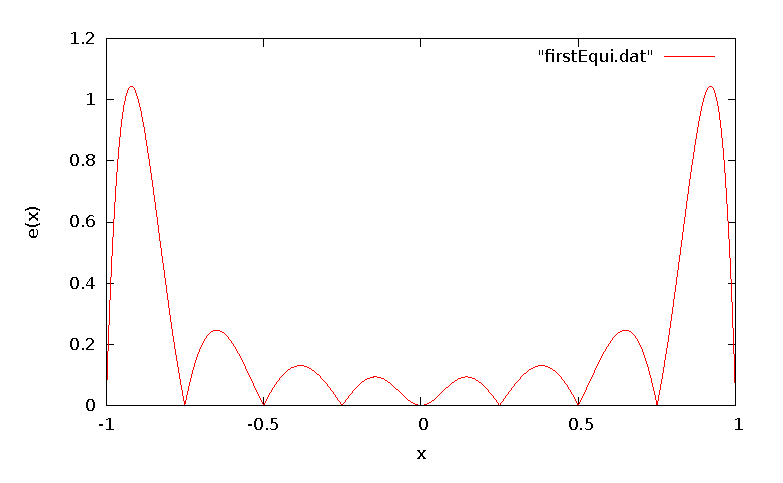
\includegraphics[width=0.8\textwidth]{wykresy/firstEqui.eps}
    \caption{Błąd interpolacji $f_1(x)$ dla węzłów równoodległych}
\end{figure}


\item $f_2(x) = \arctg x$ \\
\begin{figure}[H]
	\centering
    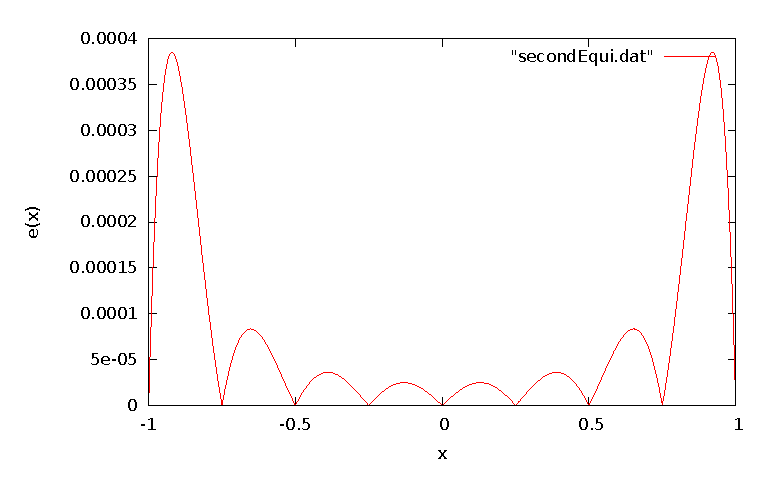
\includegraphics[width=0.8\textwidth]{wykresy/secondEqui.eps}
    \caption{Błąd interpolacji $f_2(x)$ dla węzłów równoodległych}
\end{figure}

\item $f_3(x) = \max(0, 1 - 4x)$\\
\begin{figure}[H]
	\centering
    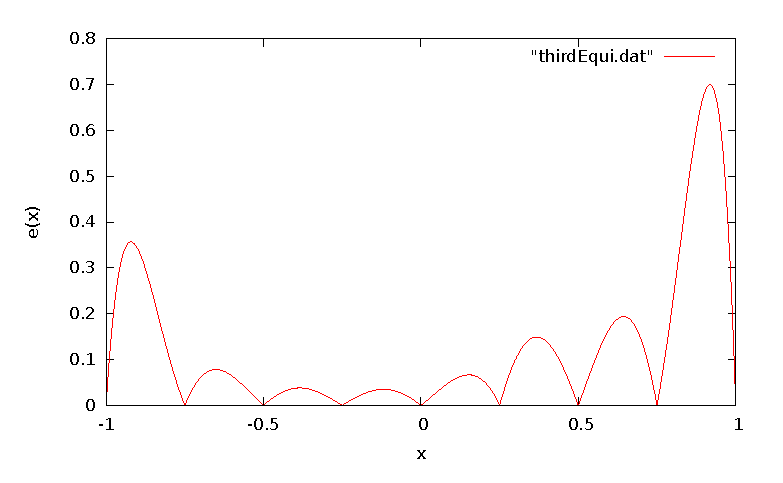
\includegraphics[width=0.8\textwidth]{wykresy/thirdEqui.eps}
    \caption{Błąd interpolacji $f_3(x)$ dla węzłów równoodległych}
\end{figure}
\end{enumerate}

\subsection{Węzły Czybyszewa}

Za węzły interpolacji wybraliśmy zera $n-tego$ wielomianu Czybyszewa. Stała Lebesgue'a przy $n = 9$ węzłach wynosi
\begin{equation*}
\Lambda_n = 2.361856787767076
\end{equation*}
Wynik ten jest zdecydowanie lepszy niż w przypadku węzłow równoodległych. Można zauważyć, że maksimum znajduje się na dwóch końcach przedziału $[-1, 1]$, tak samo jak w przypadku węzłów równoodległych.\\
Poniżej przedstawiony jest wykres stałej Lebesgue'a dla węzłów Czybyszewa. Można zauważyć logarytmiczny wzrost stałej Lebesgue'a.
\begin{figure}
    \centering
    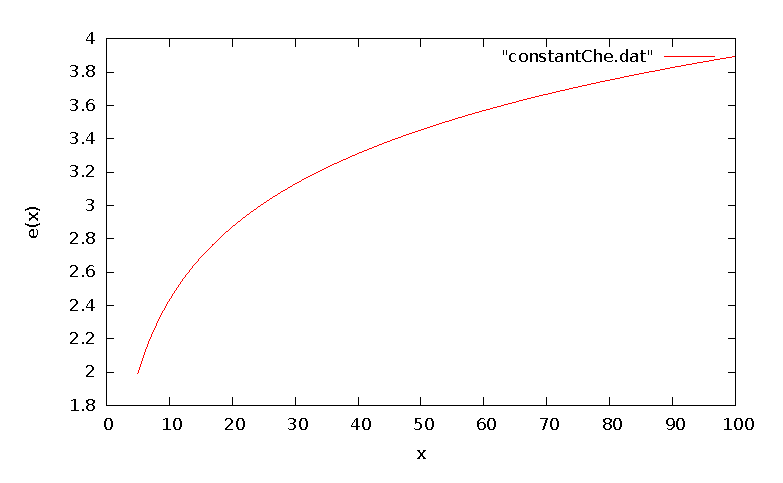
\includegraphics[width=0.8\textwidth]{wykresy/constantChe.eps}
    \caption{Stała Lebesgue'a dla węzłów Czybyszewa}
\end{figure}

\begin{enumerate}
\item $f_1(x) = \frac{1}{1 + 25x^2}$\\
\begin{figure}[H]
    \centering
    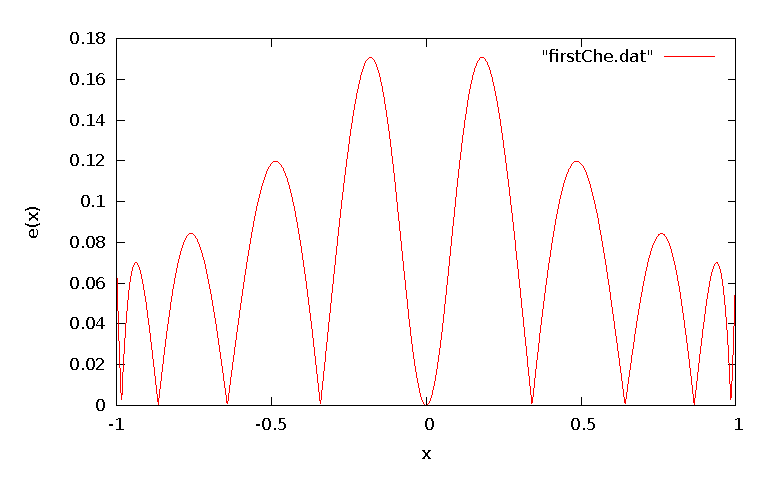
\includegraphics[width=0.8\textwidth]{wykresy/firstChe.eps}
    \caption{Błąd interpolacji $f_1(x)$ dla węzłów Czybyszewa}
\end{figure}

\item $f_2(x) = \arctg x$ \\
\begin{figure}[H]
    \centering
    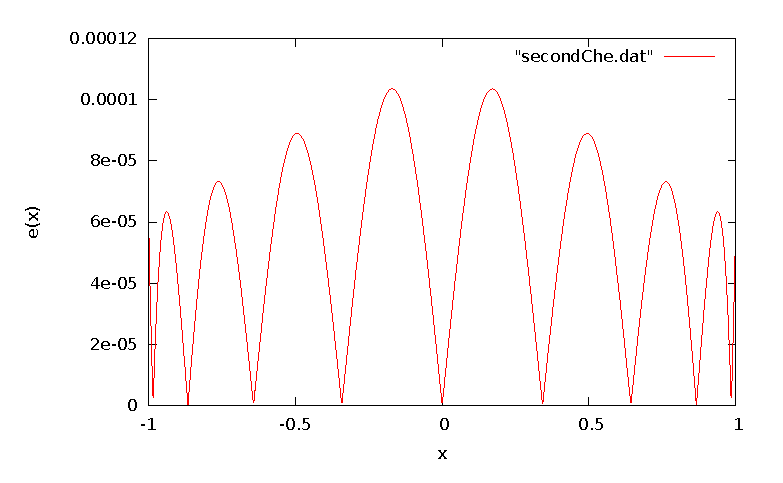
\includegraphics[width=0.8\textwidth]{wykresy/secondChe.eps}
    \caption{Błąd interpolacji $f_2(x)$ dla węzłów Czybyszewa}
\end{figure}

\item $f_3(x) = \max(0, 1 - 4x)$\\
\begin{figure}[H]
    \centering
    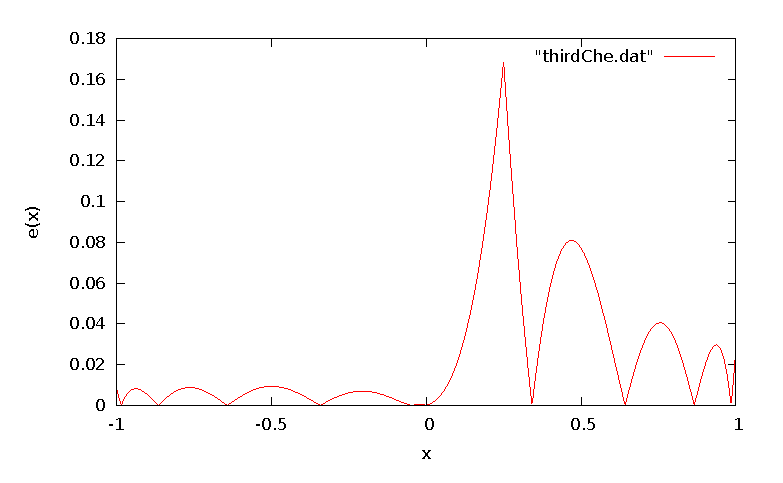
\includegraphics[width=0.8\textwidth]{wykresy/thirdChe.eps}
    \caption{Błąd interpolacji $f_3(x)$ dla węzłów Czybyszewa}
\end{figure}

\end{enumerate}

\subsection{Rozszerzone węzły Czybyszewa}
Dla $n = 9$ rozszerzonych węzłow Czybyszewa stała Lebesgue'a wynosi
\begin{equation*}
\Lambda_n = 1.9415124236504544
\end{equation*}
Jest to lepszy wynik niż dla węzłów Czybyszewa, gdzie z wykresu funkcji Lebesgue'a widać, że maksimum w przedziale $[-1, 1]$ pojawiało się zawsze na samych końcach przedziału. Teraz funkcja Lebesgue'a jest zerem dla końców przedziału.\\
Tak samo jak w przypadku zwykłych węzłów Czybyszewa, obserwujemy logarytmiczny wzrost stałej Lebesgue'a, która jest mniejsza niż stała Lebesgue'a dla węzłow Czybyszewa.
\begin{figure}
    \centering
    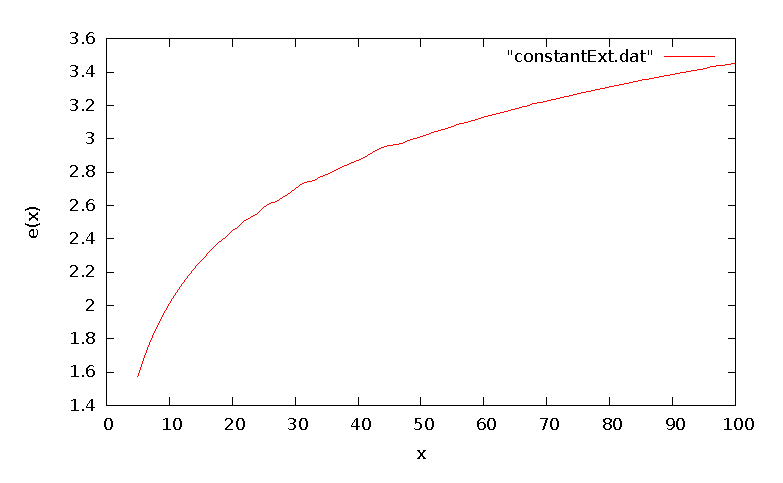
\includegraphics[width=0.8\textwidth]{wykresy/constantExt.eps}
    \caption{Stała Lebesgue'a dla rozszerzonych węzłów Czybyszewa}
\end{figure}
\begin{enumerate}
\item $f_1(x) = \frac{1}{1 + 25x^2}$\\
\begin{figure}[H]
    \centering
    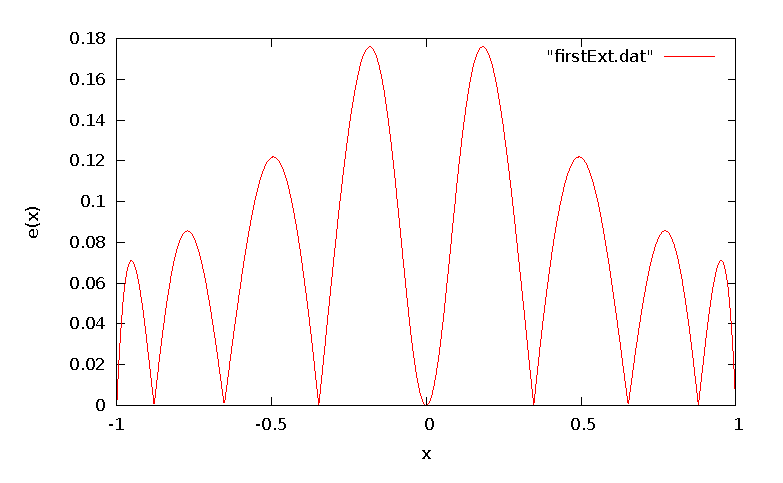
\includegraphics[width=0.8\textwidth]{wykresy/firstExt.eps}
    \caption{Błąd interpolacji $f_1(x)$ dla rozszerzonych węzłów Czybyszewa}
\end{figure}
\item $f_2(x) = \arctg x$ \\
\begin{figure}[H]
    \centering
    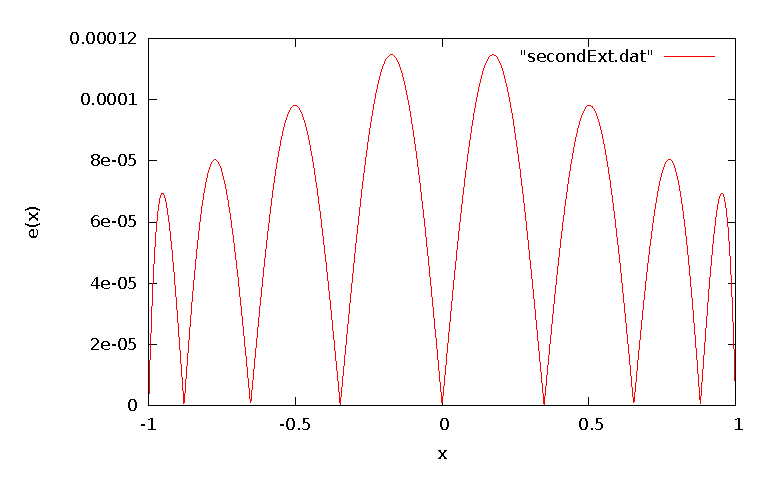
\includegraphics[width=0.8\textwidth]{wykresy/secondExt.eps}
    \caption{Błąd interpolacji $f_2(x)$ dla rozszerzonych węzłów Czybyszewa}
\end{figure}
\item $f_3(x) = \max(0, 1 - 4x)$\\
\begin{figure}[H]
    \centering
    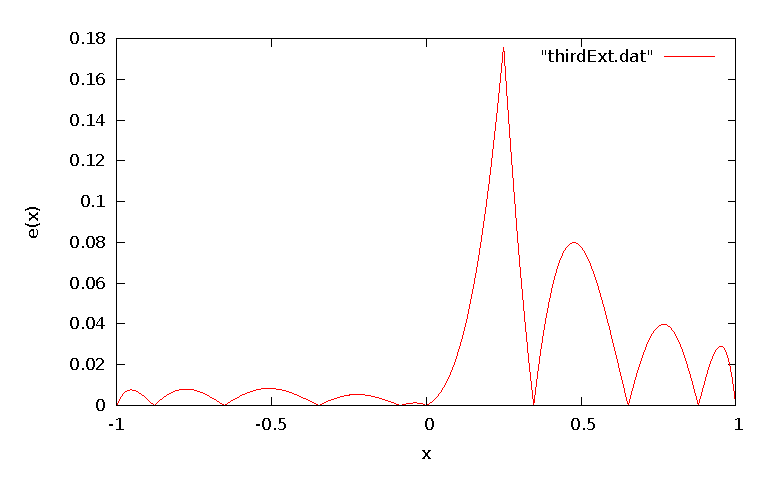
\includegraphics[width=0.8\textwidth]{wykresy/thirdExt.eps}
    \caption{Błąd interpolacji $f_3(x)$ dla rozszerzonych węzłów Czybyszewa}
\end{figure}
\end{enumerate}

\subsection{Losowe węzły}
Jak się okazuje, węzły losowe dają jeszcze gorszy wskaźnik uwarunkowania niż węzły równoodległe.
Dla dziewięciu losowo wybranych węzłów stała Lebesgue'a wyniosła
\begin{equation*}
\Lambda_n = 120.32525047803
\end{equation*}
Jest to ponad dziesięć razy wynik niż dla węzłów równoodległych.

\begin{figure}[H]
    \centering
    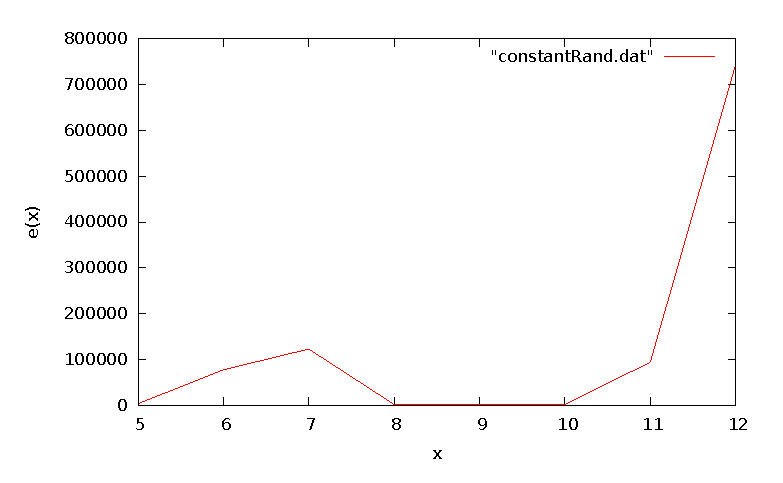
\includegraphics[width=0.8\textwidth]{wykresy/constantRand.eps}
    \caption{Stała Lebesgue'a dla losowo dobranych węzłów}
\end{figure}

Następnie wszystkie wykresy zostały przedstawione dla $n = 9$ losowych węzłów. Węzły, dla których wykresy znajdują się poniżej znajdują się w programie.
\begin{figure}[H]
    \centering
    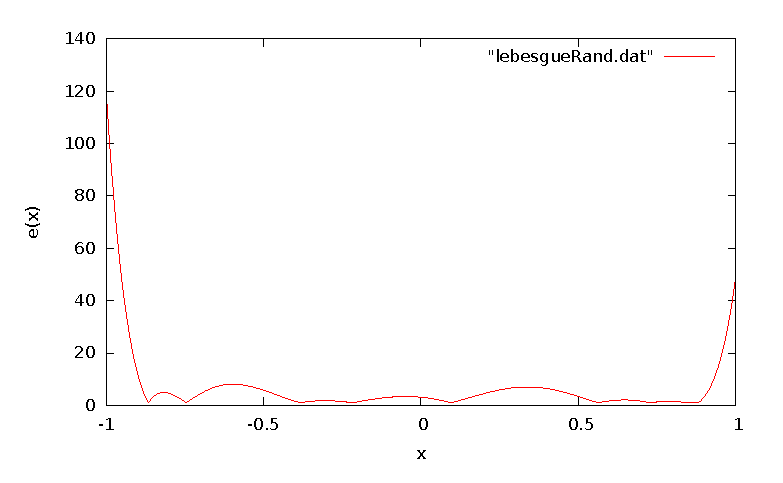
\includegraphics[width=0.8\textwidth]{wykresy/lebesgueRand.eps}
    \caption{Funkcja Lebesgue'a dla $n = 9$ losowo dobranych węzłów}
\end{figure}
W porównaniu do węzłów równoodległych funkcja Lebesgue'a jest ogromna. Stała Lebesgue'a wynosi w tym przypadku około 120.
\begin{figure}[H]
    \centering
    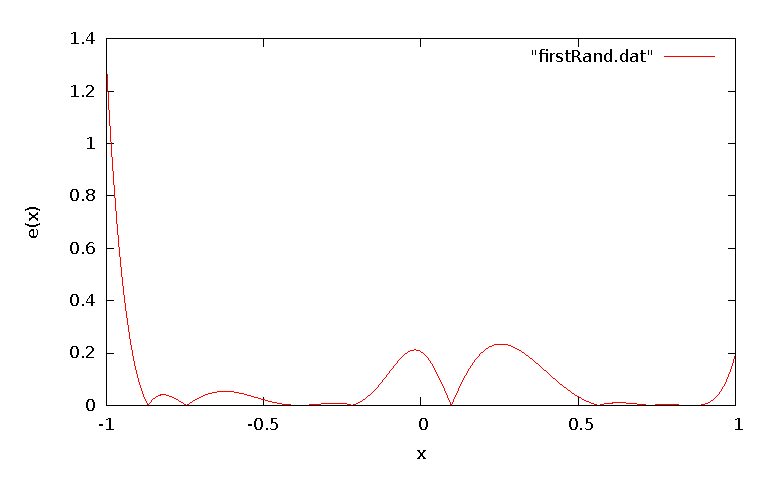
\includegraphics[width=0.8\textwidth]{wykresy/firstRand.eps}
    \caption{Błąd interpolacji $f_1(x)$ dla 9 losowo dobranych węzłów}
\end{figure}

\begin{figure}[H]
    \centering
    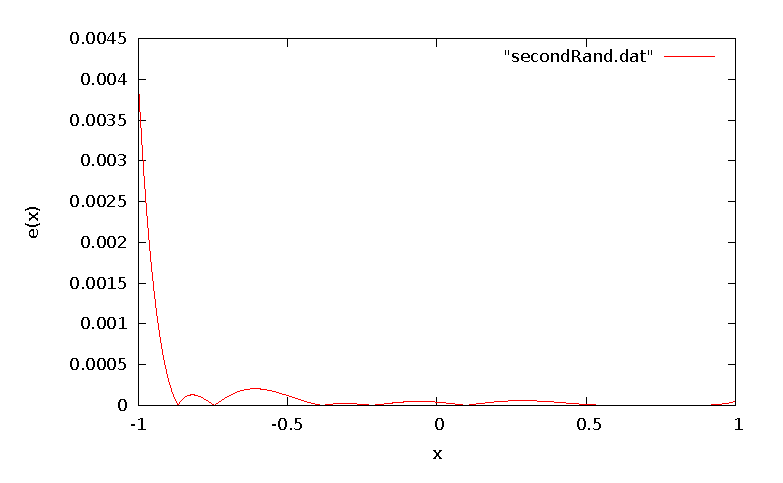
\includegraphics[width=0.8\textwidth]{wykresy/secondRand.eps}
    \caption{Błąd interpolacji $f_2(x)$ dla 9 losowo dobranych węzłów}
\end{figure}

\begin{figure}[H]
    \centering
    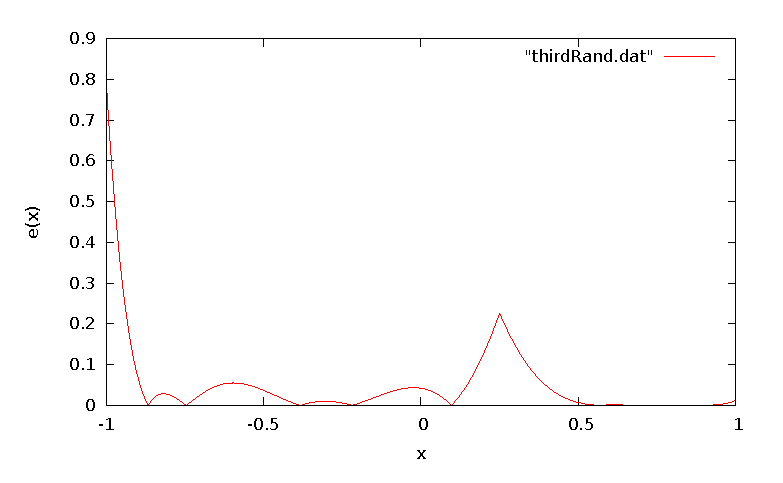
\includegraphics[width=0.8\textwidth]{wykresy/thirdRand.eps}
    \caption{Błąd interpolacji $f_3(x)$ dla 9 losowo dobranych węzłów}
\end{figure}
We wszystkich przypadkach okazało się, że losowe węzły dały o wiele większe błędy interpolacji niż pozostałe przedstawione węzły.

\section{Wnioski}

Jak się okazało, węzły losowe charakteryzują się dużym wskaźnikiem uwarunkowania oraz wysokimi błędami interpolacji w niektórych punktach.

Dla węzłów równoodległych, wielomian interpolacyjny nie odbiega zbyt bardzo od funkcji w środku przediału interpolacji, lecz na krańcach przedziału osiąga bardzo duży błąd. Dalej, jest to wynik lepszy niż dla węzłów losowych.

Węzły Czybyszewa dają niższy wskaźnik uwarunkowania oraz w niektórych punktach dają wyższe błędy interpolacji niż węzły równoodległe. Jednak w większości przedziału interpolacji węzły Czybyszewa spisują się lepiej. 

Natomiast to, że wskaźnik uwarunkowania jest wyższy, nie oznacza koniecznie tego, że błąd interpolacji także będzie wyższy. Można to zaobserwować na przykładzie węzłow Czybyszewa i rozszerzonych węzłów Czybyszewa: stała Lebesgue'a dla tych drugich węzłów jest trochę mniejsza, lecz błędy interpolacji są trochę większe. \\ Należy zaznaczyć, że wskaźnik uwarunkowania pokazuje tylko jak duże mogą być współczynniki $a_i$ w postaci potęgowej wielomianu interpolacyjnego $L_n = \sum_{i=0}^n a_i x^i$. Nawet jeśli współczynniki odbiegają znacznie od poprawnych, wyprodukowany wielomian dalej może interpolować funkcję $f$ z małymi błędami.
\begin{thebibliography}{9} 

\bibitem{Dahlquist&Bjorck}
Dahlquist, G., Bjo\"rck, A.
\emph{Numerical Methods in Scientific Computing, Volume I},
Society for Industrial and Applied Mathematics (September 4, 2008), 354-360.

\bibitem{Cheney&Light}
Cheney, E. W., Light, W. A.
\emph{A Course in Approximation Theory},
American Mathematical Soc., 2009, 11-22.

\bibitem{Erdos}
Erdo\"s, P. 
\emph{Problems and results on the theory of interpolation, II.}
Acta Math. Acad. Sci. 
Hungar. 12 (1961), 235-244.

\bibitem{Brutman}
Brutman, L.
\emph{On the Lebesgue function for polynomial interpolation.}
SIAM J. Numerical Analysis 15 (1978), 694-704.

\bibitem{Rivlin}
Rivlin, T.J.
\emph{Chebyshev Polynomials}
Wiley, New York, 1974. 2nd Edition, 1990.

\bibitem{Turetskii}
Turetskii, A. H.
\emph{The bounding of polynomials prescribed at equally distributed points.}
Proc. Pedag. Inst. Vitebsk 3 (1940), 117-127.

\bibitem{Faber}
Faber, G.
\emph{Uber die interpolatorische Darstellung stetiger Funktionen.}
Jahresber. Deutsch. Math. Verein., 23 (1914), 191-200.

\bibitem{Vertesi}
Vertesi, P.
\emph{Optimal Lebesgue constant for Lagrange interpolation.}
SIAM J. Numerical Analysis Vol. 27 (1990), 1322–1331.

\end{thebibliography}

\end{document}